
\section{Friday}\index{week8_Thursday_lecture}
\subsection{Analysis on IFT}
This lecture will talk about the full verison of IFT.
\paragraph{Elementrary Version}
Let $F: U(x_0,y_0)(\subseteq\mathbb{R}^2)\to\mathbb{R}$ be a $\mathcal{C}^p, p\ge1$ function such that
\begin{enumerate}
\item
$F(x_0,y_0)=0$,
\item
$F_y(x_0,y_0)\ne0$.
\end{enumerate}
Then we imply that there exists a neighorhood of $(x_0,y_0)$, say $I_x\times I_y$ with
\[
\begin{array}{ll}
I_x=\{x\mid |x-x_0|<\alpha\},
&
I_y=\{y\mid |y-y_0|<\beta\}
\end{array},
\]
and a unique function $f\in\mathcal{C}^p(I_x;I_y)$ such that
\begin{align*}
F(x,y)&=0\Longleftrightarrow
y=f(x),\qquad
\forall (x,y)\in I_x\times I_y\label{Eq:11:2}\\
f'(x)&=-\frac{\frac{\partial F}{\partial x}}{\frac{\partial F}{\partial y}}(x,f(x))\qquad (=-\frac{F_x}{F_y}(x,f(x))
\end{align*}

%\begin{theorem}[Elementary Version of IFT]\label{The:11:2}
%Let $F: U(x_0,y_0)(\subseteq\mathbb{R}^2)\to\mathbb{R}$ be a $\mathcal{C}^p$ ($p\ge1$) function, with
%\begin{enumerate}
%\item
%$F(x_0,y_0)=0$
%\item
%$\frac{\partial F}{\partial y}(x_0,y_0)\ne0$.
%\end{enumerate}
%Then there exists a neighborhood of $(x_0,y_0)$, say $I_x\times I_y\subseteq U(x_0,y_0)$ with
%\[
%\begin{array}{ll}
%I_x=\{x\in\mathbb{R}\mid |x-x_0|<\alpha\},
%&
%I_y=\{y\in\mathbb{R}\mid |y-y_0|<\beta\},
%\end{array}
%\]
%and an \emph{unique} function $f\in\mathcal{C}^p(I_x;I_y)$ satisfying
%\begin{align}
%F(x,y)&=0\Longleftrightarrow
%y=f(x),\qquad
%\forall (x,y)\in I_x\times I_y\label{Eq:11:2}\\
%f'(x)&=-\frac{\frac{\partial F}{\partial x}}{\frac{\partial F}{\partial y}}(x,f(x))\qquad (=-\frac{F_x}{F_y}(x,f(x)))\label{Eq:11:3}
%\end{align}
%\end{theorem}

\paragraph{Generalized version}
Let $F: U(\bm x_0,y_0)(\subseteq\mathbb{R}^m\times\mathbb{R})\to\mathbb{R}$ be a $\mathcal{C}^p,p\ge1$ function such that
\begin{enumerate}
\item
$F(\bm x_0,y_0)=0,$
\item
$F_y(\bm x_0,y_0)\ne0$.
\end{enumerate}
Then we imply that there exists a neighborhood of $(\bm x_0,y_0)$, say $I_{\bm x}\times I_y$ with
\[
\begin{array}{ll}
I_{\bm x}=\{\bm x\in\mathbb{R}^m\mid |\bm x-\bm x_0|<\alpha\},
&
I_y=\{y\in\mathbb{R}\mid |y-y_0|<\beta\},
\end{array}
\]
and a unique function $f\in\mathcal{C}^p(I_{\bm x};I_y)$ such that
\begin{align*}
F(\bm x,y)&=0\Longleftrightarrow
y = f(\bm x)\qquad \forall (\bm x,y)\in I_{\bm x}\times I_y\\
Df(\bm x)&=-\frac{1}{F_y(\bm x,f(\bm x))}D_{\bm x}F(\bm x,f(\bm x))
\end{align*}
where $Df(\bm x)=\nabla\trans f(\bm x)$, and $D_{\bm x}F(\bm x,f(\bm x))=\nabla_{\bm x}\trans F(\bm x,f(\bm x))$.

\paragraph{Full Version}
Let $F: U(\bm x_0,\bm y_0)(\subseteq\mathbb{R}^m\times\mathbb{R}^n)\to\mathbb{R}^n$ be a $\mathcal{C}^p,p\ge1$ function such that
\begin{enumerate}
\item
$F(\bm x_0,\bm y_0)=\bm 0$
\item
$D_{\bm y}F(\bm x_0,\bm y_0)$ is invertible
\end{enumerate}
Then we imply that there exists a neighborhoood of $(\bm x_0,\bm y_0)$, say $I_{\bm x}\times I_{\bm y}$, with
\[
\begin{array}{ll}
I_{\bm x}=\{\bm x\in\mathbb{R}^m\mid |\bm x-\bm x_0|<\alpha\},
&
I_{\bm y}=\{\bm y\in\mathbb{R}^n\mid |\bm y-\bm y_0|<\beta\},
\end{array}
\]
and a unique function $f\in\mathcal{C}^p(I_{\bm x};I_{\bm y})$ such that
\begin{align*}
F(\bm x,\bm y)&=0\Longleftrightarrow
\bm y = f(\bm x)\quad \forall (\bm x,\bm y)\in I_{\bm x}\times I_{\bm y}\\
Df(\bm x) &= -[D_{\bm y}F(\bm x,f(\bm x))]^{-1}D_{\bm x}F(\bm x,f(\bm x))
\end{align*}
where $Df(\bm x)\in\mathbb{R}^{n\times m}$; $D_{\bm y}F(\bm x,f(\bm x))\in\mathbb{R}^{n\times n}$; and $D_{\bm x}F(\bm x,f(\bm x))\in\mathbb{R}^{n\times m}$.
\begin{proof}
Fix $m$, induction on $n$.
\begin{enumerate}
\item
As $n=1$, it is done.
\item
The rest are similar to the proof in elementary version.
\end{enumerate}
Check the detail in Zorich's book from Page 490 to Page 494.
\end{proof}
\begin{remark}
Pay attention to the order of matrix multiplication and the matrix size when applying full version IFT.
\end{remark}
\subsection{Applications on IFT}
\paragraph{When does a mapping has its inverse locally?}
Firstly, we aim to answer two questions:
\begin{enumerate}
\item
When does a mapping has its inverse?
\item
What is the derivative of the mapping's inverse?
\end{enumerate}
\begin{definition}[diffeomorphism]
A mapping $f:U(\subseteq\mathbb{R}^m)\to V\subseteq\mathbb{R}^m$ is called a $\mathcal{C}^p$-diffeomorphism $(p=0,1,2,\dots)$ if
\begin{enumerate}
\item
$f\in\mathcal{C}^p(U;V)$;
\item
$f$ is a bijection
\item
$f^{-1}\in\mathcal{C}^p(U;V)$
\end{enumerate}
\end{definition}

\begin{theorem}[Inverse Function Theorem]
If the function $f:E\to\mathbb{R}^m$, with $E$ to be a \emph{domain} (pre-assume its connectedness) in $\mathbb{R}^m$, is such that
\begin{enumerate}
\item
$f\in\mathcal{C}^p(E;\mathbb{R}^m), p\ge1$
\item
$\bm y_0=f(\bm x_0)$ for a $\bm x_0\in E$
\item
$Df(\bm x_0)$ is invertible, where $\bm x_0\in E$
\end{enumerate}
Then we imply that
\begin{enumerate}
\item
$f$ is invertible near $\bm x_0$. Furthermore, there exists a neighborhood of $(\bm x_0,\bm y_0)$, say $U(\bm x_0)\times V(\bm y_0)$ such that $f: U(\bm x_0)\to V(\bm y_0)$ is a $\mathcal{C}^p$-diffeomorphism
\item
Suppose $g=f^{-1}: V(\bm y_0)\to U(\bm x_0)$, then
\[
Dg(\bm y)=[Df(g(\bm y))]^{-1}
\]
\end{enumerate}
\end{theorem}
\begin{proof}
Construct a function 
\begin{equation}\label{Eq:11:15}
F(\bm x,\bm y): f(\bm x)-\bm y=\bm0\mbox{ with $F:E\times\mathbb{R}^m\to\mathbb{R}^m$}
\end{equation}
It suffices to solve $F(\bm x,\bm y)=0$ w.r.t. $\bm x$. It is easy to verify that
\begin{subequations}
\begin{align}
F&\in\mathcal{C}^p(E\times\mathbb{R}^m;\mathbb{R}^m),\quad p\ge1;\\
F(\bm x_0,\bm y_0)&=0;\\
D_{\bm x}F(\bm x_0,\bm y_0) &= Df(\bm x_0)\mbox{ is invertible},
\end{align}
\end{subequations}
i.e., the hypotheses of IFT is satisfied. By applying IFT, we imply that there exists a neighborhood $I_{\bm x}=\{\bm x\in E\mid |\bm x-\bm x_0|<\alpha\}$ and $I_{\bm y}=\{\bm y\in\mathbb{R}^m\mid |\bm y-\bm y_0|<\beta\}$ and $g\in\mathcal{C}^p(I_{\bm y};I_{\bm x})$ such that
\begin{subequations}
\begin{align}
F(\bm x,\bm y)&=0\Longleftrightarrow
\bm x=g(\bm y),\quad\forall (\bm x,y)\in I_{\bm x}\times I_{\bm y}\label{Eq:11:17:a}\\
Dg(\bm y)&=-[D_{\bm x}F(g(\bm y), \bm y)]^{-1}D_{\bm y}F(g(\bm y),\bm y).	\label{Eq:11:17:b}
\end{align}
\end{subequations}

Substituting (\ref{Eq:11:17:a}) into (\ref{Eq:11:15}), we derive that $f(g(\bm y))=\bm y$ iff $\bm x=g(\bm y)$, i.e., $g$ is $\mathcal{C}^p$-diffeomorphism, i.e., $f$ is $\mathcal{C}^p$-diffeomorphism.

Also, note that $D_{\bm y}F(g(\bm y),\bm y)=-\bm I$, and substituting it into (\ref{Eq:11:17:b}), we derive
\[
Dg(\bm y)=[Df(\bm x)]^{-1}
\]
\end{proof}


\paragraph{
When does a vector function admits its canonical form?
}
In linear algebra we have learnt various ways of decomposition. One of the most useful one is SVD decomposition, i.e., a matrix $\bm A$ can be decomposed as $\bm U\bm\Sigma\bm V$, where 
\begin{enumerate}
\item
$\bm\Sigma$ is a matrix with zeros on the off-diagonal, and $r$ non-zero entries on the diagonal $(r=\rank(\bm A))$. 
\item
$\bm U$ and $\bm V$ are unitary matrices satisfying $\bm U\bm U\trans=\bm I;\bm V\bm V\trans=\bm I$.
\end{enumerate}
We can say that any matrix admits its SVD canonical form. We aim to generalize it into functional space.

\paragraph{Notations and Conventions}
The proof of the functional rank theorem may be messy. To simplify it, we adopt the notation $\frac{\partial (f_1,\dots,f_m)}{\partial (x_1,\dots,x_n)}$ to denote the Jacobian matrix of $f:\mathbb{R}^n\to\mathbb{R}^m$. Also, we define the generlized rank for a vector function (may be non-linear):
\begin{definition}[Rank]
The \emph{rank} of a vector function $f:U(\subseteq\mathbb{R}^m)\to\mathbb{R}^n$ at a point $\bm x\in U$ is defined to be the \textit{rank} of $Df(\bm x)$.
\end{definition}
%
\begin{theorem}[Rank Theorem]\label{The:11:5}
Let $f: U(\bm x_0) (\subseteq\mathbb{R}^m)\to\mathbb{R}^n$ be a function such that
\begin{enumerate}
\item
$\bm y_0:=f(\bm x_0)$;
\item
$f\in\mathcal{C}^p(U(\bm x_0);\mathbb{R}^n)$;
\item
$f$ has the same constant rank $k$ for $\forall\bm x\in U(\bm x_0)$;
\end{enumerate}
then there exists a neighborhood of $(\bm x_0,\bm y_0)$, say $N(\bm x_0)\times N(\bm y_0)$, and two $\mathcal{C}^p-$ diffeomorphism with
\[
\begin{array}{ll}
\mbox{$\bm u=\phi(\bm x)$ for $\bm x\in N(\bm x_0)$,}
&
\mbox{$\bm v=\psi(\bm y)$ for $\bm y\in N(\bm y_0)$,}
\end{array}
\]
such that the mapping $\bm v = \psi\circ f\circ\phi^{-1}(\bm u)$ takes the form
\[
\bm u:=(u_1,\dots,u_k,u_{k+1},\dots,u_m)\mapsto
\bm v=(v_1,\dots,v_n):=(u_1,\dots,u_k,0,\dots,0)
\]
\end{theorem}
\begin{remark}
In other words, the theorem asserts that if given the mapping $\bm y=f(\bm x)$ and if the hypotheses in Theorem~(\ref{The:11:5}) are satisfied, then there exists one way of change of variable $\bm u=\phi(\bm x), \bm v=\psi(\bm y)$, such that the mapping induced from the change of variable $\bm v = \psi\circ f\circ\phi^{-1}(\bm u)$ has the coordinate representation
\[
\bm u:=(u_1,\dots,u_k,u_{k+1},\dots,u_m)\mapsto\bm v:=
(u_1,\dots,u_k,0,0,\dots,0).
\]
\begin{figure}[H]
\centering
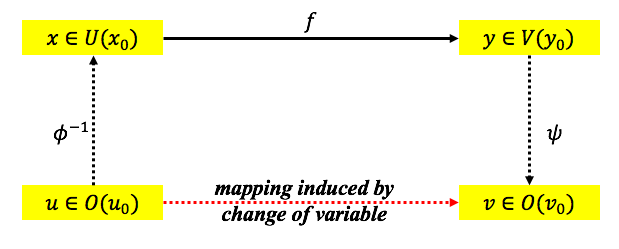
\includegraphics[width=14cm]{week11/F_11_3}
\caption{The canonical form representation of $\psi\circ f\circ\phi^{-1}$}
\end{figure}
\end{remark}

\textit{Proof:}
\paragraph{Step 1: Show that the $k$-th order principal minor of Jacobian matrix is non-singular on some neighborhood}
Since $\rank(Df(\bm x_0))=k$, by re-ordering the coordinates, we can assume that the $k$-th order principal minor, say $\frac{\partial (f_1,\dots,f_k)}{\partial (x_1,\dots,x_k)}(\bm x_0)$ has $k$ independent columns, i.e., non-singular. Due to the continuity of matrix function $\det(\cdot)$ and $\mathcal{C}^p$ function $f$, we imply that $\rank(Df(\bm x))=k$ for $\bm x$ in some neighborhood of $\bm x_0$.

\paragraph{Step 2: Construct a $\mathcal{C}^p$-diffeomorphism $\phi$}
Construct a mapping $\phi$ defined in $U(\bm x_0)$:
\begin{equation}\label{Eq:11:18}
\begin{pmatrix}
u_1\\\vdots\\u_k\\u_{k+1}\\\vdots\\u_m
\end{pmatrix}
=
\phi(\bm x)
=\begin{pmatrix}
f_1(\bm x)\\
\vdots\\
f_k(\bm x)\\
x_{k+1}\\
\vdots\\
x_m
\end{pmatrix}
\end{equation}

Whether this mapping has its inverse? The Jacobian matrix of $\phi$ for $\bm x\in U(\bm x_0)$ is given by:
\[
\bm J=\begin{pmatrix}
\frac{\partial (f_1,\dots,f_k)}{\partial(x_1,\dots,x_k)}&\frac{\partial {f_1,\dots,f_k}}{\partial (x_{k+1},\dots,x_m)}\\
\bm0&\bm I
\end{pmatrix}_{[k+(m-k)]\times [k+(m-k)]},
\]
with the determinant $|\bm J|=|\frac{\partial (f_1,\dots,f_k)}{\partial(x_1,\dots,x_k)}|\cdot|\bm I|\ne0$, i.e., the mapping $\phi(\bm x_0)$ has non-singular Jacobian matrix. 

By applying inverse function theorem, we derive that $\phi(\bm x)$ is a $\mathcal{C}^p$-diffeomorphism on $N(\bm x_0)$, where $N(\bm x_0)$ is some neighborhood of $\bm x_0$.

\paragraph{Step 3: Study the mapping $f\circ\phi^{-1}$}
Considering the relation (\ref{Eq:11:18}), we can see the mapping $g:=f\circ\phi^{-1}$ has the representation:
\begin{equation}\label{Eq:11:19}
\begin{pmatrix}
y_1\\\vdots\\y_k\\y_{k+1}\\\vdots\\y_n
\end{pmatrix}=f\circ\phi^{-1}(\bm u)=\begin{pmatrix}
u_1\\\vdots\\u_k\\g_{k+1}(u_1,\dots,u_m)\\\vdots\\g_n(u_1,\dots,u_m)
\end{pmatrix}
\end{equation}

On the one hand, its Jacobian matrix by chain rule is given by $Dg(\bm u)=Df(\phi^{-1}(\bm u))* D\phi^{-1}(\bm u)$, with $\rank(Df(\phi^{-1}(\bm u)))=\rank(Df(\bm u))=m$ and $\rank(D\phi^{-1}(\bm u))\le m$. Applying the relation $\rank(\bm{AB})=\rank(\bm A)$ for invertible $\bm B$, we derive that the matrix $Dg(\bm u)$ has rank $k$ for every point $\bm u\in\phi(N(\bm x_0))$.

On the other hand, direct computation of the Jacobian matrix for the mapping (\ref{Eq:11:19}) yields
\[
Dg(\bm u)=\begin{bmatrix}
\bm I&\bm0\\
\frac{\partial(g_{k+1},\dots,g_n)}{\partial(u_1,\dots,u_k)}
&
\frac{\partial(g_{k+1},\dots,g_n)}{\partial(u_{k+1},\dots,u_m)}
\end{bmatrix}_{[k+(n-k)]\times[(k+(m-k)]}
\]
Since $\rank(Dg(\bm u))=k$, we conclude that $\frac{\partial(g_{k+1},\dots,g_n)}{\partial(u_{k+1},\dots,u_m)}$ is a zero matrix, which implies that $(g_{k+1},\dots,g_n)$ is independent of $(u_{k+1},\dots,u_m)$. Thus the mapping (\ref{Eq:11:19}) can be re-written as:
\begin{equation}\label{Eq:11:20}
\begin{pmatrix}
y_1\\\vdots\\y_k\\y_{k+1}\\\vdots\\y_n
\end{pmatrix}=f\circ\phi^{-1}(\bm u)=\begin{pmatrix}
u_1\\\vdots\\u_k\\g_{k+1}(u_1,\dots,u_k)\\\vdots\\g_n(u_1,\dots,u_k)
\end{pmatrix}
\end{equation}

\paragraph{Step 4: Construct a $\mathcal{C}^p$-diffeomorphism $\psi$}
Construct a mapping $\psi$ defined in a neighborhood of $\bm y_0$, say $\hat N(\bm y_0)$:
\begin{equation}\label{Eq:11:21}
\begin{pmatrix}
v_1\\\vdots\\v_k\\v_{k+1}\\\vdots\\v_n
\end{pmatrix}=\psi(\bm y)=\begin{pmatrix}
y_1\\\vdots\\y_k\\y_{k+1}-g_{k+1}(y_1,\dots,y_k)\\\vdots\\y_n-g_n(y_1,\dots,y_k)
\end{pmatrix}
\end{equation}
It's clear that the mapping $\psi$ is a $\mathcal{C}^p$ function in $N(\bm y_0)$, and its Jacobian matrix has the form:
\[
D\psi(\bm y_0)=\begin{bmatrix}
\bm I&\bm0\\
-\frac{\partial(g_{k+1},\dots,g_n)}{\partial(y_1,\dots,y_k)}&\bm I
\end{bmatrix},
\]
which has the determinant 1, i.e., is non-singular.

Applying inverse function theorem, we derive that $\phi(\bm y_0)$ is $\mathcal{C}^p$-diffeomorphism on $N(\bm t_0)$, where $N(\bm y_0)\subseteq \hat N(\bm y_0)$ is some neighborhood of $\bm y_0$.
\paragraph{Step 5: Study the mapping $\psi\circ f\circ\phi^{-1}$}
Hence, $\psi\circ f\circ\phi^{-1}=\psi\circ g$. Applying the relation (\ref{Eq:11:20}) and (\ref{Eq:11:21}), we see that the mapping $\psi\circ g$ has the canonical representation:
\[
\psi\circ g\begin{pmatrix}
u_1\\\vdots\\u_k\\u_{k+1}\\\vdots\\u_m
\end{pmatrix}=
\psi\begin{pmatrix}
u_1\\\vdots\\u_k\\g_{k+1}(u_1,\dots,u_k)\\\vdots\\g_n(u_1,\dots,u_k)
\end{pmatrix}=
\begin{pmatrix}
u_1\\\vdots\\u_k\\0\\\vdots\\0
\end{pmatrix}
\]
The proof is complete.

\paragraph{Application: What is the dimension of a sphere $\mathbb{S}^2\subseteq\mathbb{R}^3$?}
Define the dimension for the plane $\{(x,y,0)\mid (x,y)\in [a,b]\times[c,d]\}$ is 2. What is the dimension of the sphere 
\[\mathbb{S}^2=
\{(\sin\phi\cos\theta,\sin\phi\sin\theta,\cos\theta)\mid \phi\in[0,\pi),\theta\in[0,2\pi)\}
\]
Define the mapping $F(\phi,\theta)=(\sin\phi\cos\theta,\sin\phi\sin\theta,\cos\theta)$ over the domain $[0,\pi)\times[0,2\pi)$. It's easy to verify that $\rank(F)=2$. Thus for any point $(\phi,\theta)\in[0,\pi)\times[0,2\pi)$, by rank theorem, there exists a way of change of variable such that the mapping $f$ can be transformed as:
\[
(u_1,u_2)\mapsto(u_1,u_2,0),
\]
i.e., that curved sphere can be bijectively mapped into a flat 2-dimension plane. Thus $\dim(\mathbb{S}^2)=2$.


\paragraph{Comments on Quiz and Final}
The quiz and final will emphasis the importance of computation as well, e.g., \textit{how to apply chain rule to differentiate?}, \textit{how to compute Jacobian matrix, and the inverse?} On the remaining Wednesday, we will continue to discuss the application of IFT.
















